\documentclass[xcolor=dvipsnames, 10pt]{beamer}  



\setbeamertemplate{navigation symbols}

\mode<presentation>
{
  \usetheme{Singapore}
  % or ...
  \setbeamercovered{transparent}
  % or whatever (possibly just delete it)
}


%\renewcommand{\insertnavigation}[1]{}
%
\addtobeamertemplate{navigation symbols}{}{%
    \usebeamerfont{footline}%
    \usebeamercolor[fg]{footline}%
    \hspace{1em}%
    \insertframenumber/\inserttotalframenumber
    \vspace{0.5em}
}


\setbeamercolor{footline}{fg=blue}
\setbeamerfont{footline}{series=\bfseries}

\AtBeginDocument{%
      \DeclareSymbolFont{pureletters}{T1}{lmr}{\mddefault}{it}%
      }
      
\usepackage{amsmath, amssymb, amsthm}

\usepackage{tikz}
\usetikzlibrary{positioning, arrows.meta}
\usetikzlibrary{patterns}
\usetikzlibrary{backgrounds}
\usetikzlibrary{shadows}

\usepackage{diagbox}
\usepackage{tabularx}
\usepackage{graphicx}
\usepackage{xcolor}
\usepackage{pifont}
\usepackage{listings}
\usepackage{balance}
\usepackage{lipsum}
\usepackage{indentfirst}
\usepackage{subcaption}
%\usepackage[utf8]{inputenc}  % Not needed with XeLaTeX/LuaLaTeX
\usepackage{fontspec}
\setmonofont{DejaVu Sans Mono}[Scale=MatchLowercase]
%\newfontfamily{\emojifont}{Noto Color Emoji}
\usepackage{algorithm}
\usepackage{algorithmic}
%\usepackage[linesnumbered,ruled,vlined]{algorithm2e}
%\usepackage{algpseudocode}
\usepackage{booktabs}

\usepackage[xcharter]{newtxmath}
\usepackage[mathscr]{}
\usepackage{stmaryrd} % St Mary's Road symbols font --- some extra symbols
\usepackage{bbm}
\usepackage{centernot}

\usepackage[font=scriptsize]{caption}
\setbeamertemplate{caption}[numbered]

\usepackage{pgfplots}
\usepgfplotslibrary{fillbetween}

\usepackage{ragged2e}
\usepackage{varwidth}

\usepackage{hyperref} 
\definecolor{darkblue}{rgb}{0,0,.6}
\definecolor{darkred}{rgb}{0.55, 0, 0}


\usepackage[sort&compress]{natbib}
% removes reference from top menu bar
\renewcommand\bibsection{\section[]{\refname}}
% remove roman numbering for nobreak references
\setbeamertemplate{frametitle continuation}{}

% change the color of the citation and ref
\bibpunct{\textcolor{darkblue}{(}}{\textcolor{darkblue}{)}}{,}{a}{}{;}
\renewcommand{\eqref}[1]{\textcolor{darkblue}{(}\ref{#1}\textcolor{darkblue}{)}}

\definecolor{codebg}{RGB}{241, 241, 241}
\definecolor{dogerblue}{RGB}{24,116,205}
\definecolor{blue2}{RGB}{0,0,238}
\definecolor{bg}{rgb}{0.95,0.95,0.95}
\definecolor{DarkOrange1}{RGB}{255,127,0}
\definecolor{ForestGreen}{RGB}{34,139,34}
\definecolor{DarkRed}{RGB}{139, 0, 0}
\definecolor{DarkBlue}{RGB}{0, 0, 139}
\definecolor{Blue}{RGB}{0, 0, 255}
\definecolor{Brown}{RGB}{165,42,42}



% Hyperref setup for colored links
\hypersetup{colorlinks=true,citecolor=darkblue,linkcolor=darkblue,urlcolor=blue}

\newcommand{\assumptionref}[1]{\hyperlink{#1}{Assumption~\ref*{#1}}}
\newcommand{\theoremref}[1]{\hyperlink{#1}{Theorem~\ref*{#1}}}
\newcommand{\lemmaref}[1]{\hyperlink{#1}{Lemma~\ref*{#1}}}
\newcommand{\propositionref}[1]{\hyperlink{#1}{Proposition~\ref*{#1}}}
\newcommand{\exampleref}[1]{\hyperlink{#1}{Example~\ref*{#1}}}
\newcommand{\definitionref}[1]{\hyperlink{#1}{Definition~\ref*{#1}}}
\newcommand{\resultref}[1]{\hyperlink{#1}{Result~\ref*{#1}}}
\newcommand{\figref}[1]{\hyperlink{#1}{Figure~\ref*{#1}}}

\usepackage[cache=true, cachedir=_minted]{minted}
\usemintedstyle{friendly}
\setminted[python]{
  fontsize=\small,
  baselinestretch=1.2,
  linenos=false,
  breaklines=true,
  frame=none
}


\usepackage[most]{tcolorbox}
\tcbuselibrary{theorems}

\newtcbtheorem{TheoremBox}{Theorem}{
    enhanced,
    fontupper=\small\sffamily,
    colback=white,
    colframe=red!55!black,
    left=1mm,
    right=1mm,
    top=1mm,
    bottom=1mm
}{th}

% Reset theorem counter on overlays to prevent incrementing with \pause
\resetcounteronoverlays{tcb@cnt@TheoremBox}

\newtcbtheorem{PropositionBox}{Proposition}{
    enhanced,
    fontupper=\small\sffamily,
    colback=white,
    colframe=blue!45!yellow,
    left=1mm,
    right=1mm,
    top=1mm,
    bottom=1mm
}{pr}

\resetcounteronoverlays{tcb@cnt@PropositionBox}

\newtcbtheorem{AssumptionBox}{Assumption}{
    enhanced,
    fontupper=\small\sffamily,
    colback=white,
    colframe=yellow!45!black,
    left=1mm,
    right=1mm,
    top=1mm,
    bottom=1mm
}{as}

\resetcounteronoverlays{tcb@cnt@AssumptionBox}

\newtcbtheorem{ExampleBox}{Example}{
    enhanced,
    fontupper=\small\sffamily,
    colback=white,
    colframe=green!35!blue,
    left=1mm,
    right=1mm,
    top=1mm,
    bottom=1mm
}{ex}

\resetcounteronoverlays{tcb@cnt@ExampleBox}

\newtcbtheorem{ResultBox}{Result}{
  enhanced,
  fontupper=\small\sffamily,  
  colback=white,
  colframe=red!90!black!75,
  left=1mm,
  right=1mm,
  top=1mm,
  bottom=1mm
}{re}

\resetcounteronoverlays{tcb@cnt@ResultBox}

\newtcbtheorem{DefinitionBox}{Definition}{
  enhanced,
  fontupper=\small\sffamily,
  colback=white,
  colframe=blue!45!black,
  left=1mm,
  right=1mm,
  top=1mm,
  bottom=1mm
}{de}

\resetcounteronoverlays{tcb@cnt@DefinitionBox}

\newtcbtheorem{CorollaryBox}{Corollary}{
  enhanced,
  fontupper=\small\sffamily,
  colback=white,
  colframe=brown!45!black,
  left=1mm,
  right=1mm,
  top=1mm,
  bottom=1mm
}{co}

\resetcounteronoverlays{tcb@cnt@CorollaryBox}

\newtcbtheorem{LemmaBox}{Lemma}{
  enhanced,
  fontupper=\small\sffamily,
  colback=white,
  colframe=brown!45!black,
  left=1mm,
  right=1mm,
  top=1mm,
  bottom=1mm
}{co}

\resetcounteronoverlays{tcb@cnt@LemmaBox}

\setbeamertemplate{theorems}[numbered]
\newtheorem{thm}{Theorem}
\newtheorem{lem}[thm]{Lemma}
\newtheorem{cor}[thm]{Corollary}
\newtheorem{rem}[thm]{Remark}
\newtheorem{remark}[thm]{Remark}
\newtheorem{conj}[thm]{Conjecture}
\newtheorem{defn}[thm]{Definition}
\newtheorem{prop}[thm]{Proposition}
\newtheorem{ill}[thm]{Illustration}

% nice inequalities
\renewcommand{\leq}{\leqslant}
\renewcommand{\geq}{\geqslant}

% inner product
\providecommand{\inner}[1]{\left\langle{#1}\right\rangle}
\providecommand{\innerp}[1]{\left\langle{#1}\right\rangle_\pi}


%extra spacing
\renewcommand{\baselinestretch}{1.2}


%horizonal line
\newcommand{\HRule}{\rule{\linewidth}{0.3mm}}

% skip a line between paragraphs, no indentation
\setlength{\parskip}{1.5ex plus0.5ex minus0.5ex}
\setlength{\parindent}{0pt}

% footnote without a maker (blfootnote)
\newcommand\blfootnote[1]{%
  \begingroup
  \renewcommand\thefootnote{}\footnote{#1}%
  \addtocounter{footnote}{-1}%
  \endgroup
}

\DeclareMathOperator{\Span}{span}
\DeclareMathOperator{\diag}{diag}
\DeclareMathOperator*{\argmin}{arg\,min}
\DeclareMathOperator*{\argmax}{arg\,max}

\DeclareMathOperator{\cl}{cl}
\DeclareMathOperator{\Int}{int}
%\DeclareMathOperator{\overset{\circ}}{int}
\DeclareMathOperator{\Prob}{Prob}
\DeclareMathOperator{\determinant}{det}
\DeclareMathOperator{\Var}{Var}
\DeclareMathOperator{\Cov}{Cov}
\DeclareMathOperator{\graph}{graph}

\definecolor{Brown}{rgb}{0.59, 0.29, 0.0}
\definecolor{backgroundgray}{RGB}{240, 240, 240}
\definecolor{containerblue}{RGB}{70, 130, 180}
\definecolor{leafgreen}{RGB}{60, 179, 113}
\definecolor{textgray}{RGB}{80, 80, 80}


\newcommand{\Eg}{\textcolor{Brown}{Eg. }}
\newcommand{\Def}{\textcolor{Brown}{Def. }}
\newcommand{\Egs}{\textcolor{Brown}{Egs. }}

% mics short cuts and symbols
\newcommand{\too}{\stackrel { o } {\to} }
\newcommand{\st}{\ensuremath{\ \mathrm{s.t.}\ }}
\newcommand{\setntn}[2]{ \{ #1 : #2 \} }
\newcommand{\fore}{\therefore \quad}
\newcommand{\preqsd}{\preceq_{sd} }
\newcommand{\toas}{\stackrel {\textrm{ \scriptsize{a.s.} }} {\to} }
\newcommand{\tod}{\stackrel { d } {\to} }
\newcommand{\tou}{\stackrel { u } {\to} }
\newcommand{\toweak}{\stackrel { w } {\to} }
\newcommand{\topr}{\stackrel { p } {\to} }
\newcommand{\disteq}{\stackrel { \mathscr D } {=} }
\newcommand{\eqdist}{\stackrel {\textrm{ \scriptsize{d} }} {=} }
\newcommand{\iidsim}{\stackrel {\textrm{ {\sc iid }}} {\sim} }
\newcommand{\1}{\mathbbm 1}
\newcommand{\la}{\langle}
\newcommand{\ra}{\rangle}
\newcommand{\dee}{\,{\rm d}}
\newcommand{\og}{{\mathbbm G}}
\newcommand{\ctimes}{\! \times \!}
\newcommand{\sint}{{\textstyle\int}}

\newcommand{\given}{\, | \,}
\newcommand{\A}{\forall}

% d for integrals
\newcommand*\diff{\mathop{}\!\mathrm{d}}
\newcommand*\e{\mathrm{e}}


% Special symbols and shortcuts
\newcommand{\bmeta}{\bm{\eta}}
\newcommand{\bmxi}{\bm{\xi}}

\newcommand{\infot}{\fF_t}

\newcommand{\pspace}{\mathscr{P}(\mathsf{X})}
\newcommand{\cspace}{\mathscr{C}(\mathsf{X})}

%\renewcommand{\times}{\! \times \!}

\newcommand{\aA}{\mathcal A}
\newcommand{\bB}{\mathscr B}
\newcommand{\cC}{\mathscr C}
\newcommand{\dD}{\mathcal D}
\newcommand{\sS}{\mathscr S}
\newcommand{\oO}{\mathcal O}
\newcommand{\gG}{\mathcal G}
\newcommand{\hH}{\mathcal H}
\newcommand{\kK}{\mathcal K}
\newcommand{\iI}{\mathcal I}
\newcommand{\eE}{\mathcal E}
\newcommand{\fF}{\mathscr F}
\newcommand{\qQ}{\mathcal Q}
\newcommand{\tT}{\mathcal T}
\newcommand{\xX}{\mathcal X}
\newcommand{\yY}{\mathcal Y}
\newcommand{\rR}{\mathcal R}
\newcommand{\zZ}{\mathcal Z}
\newcommand{\wW}{\mathcal W}
\newcommand{\uU}{\mathcal U}
\newcommand{\lL}{\mathcal L}

\newcommand{\mM}{\mathcal M}


\newcommand{\vV}{\mathcal V}

\newcommand{\Bsf}{\mathsf B}
\newcommand{\Hsf}{\mathsf H}
\newcommand{\Vsf}{\mathsf V}

\newcommand{\BB}{\mathbbm B}
\newcommand{\DD}{\mathbbm D}
\newcommand{\RR}{\mathbbm R}
\newcommand{\CC}{\mathbbm C}
\newcommand{\QQ}{\mathbbm Q}
\newcommand{\NN}{\mathbbm N}
\newcommand{\GG}{\mathbbm G}
\newcommand{\UU}{\mathbbm U}
\newcommand{\TT}{\mathbbm T}
\newcommand{\YY}{\mathbbm Y}
\newcommand{\ZZ}{\mathbbm Z}
\newcommand{\HH}{\mathbbm H}
\newcommand{\MM}{\mathbbm M}
\newcommand{\PP}{\mathbbm P}
\newcommand{\EE}{\mathbbm E}


\newcommand{\bH}{\mathbf H}
\newcommand{\bT}{\mathbf T}

\newcommand{\var}{\mathbbm V}

\newcommand{\Asf}{\mathsf A}
\newcommand{\Gsf}{\mathsf G}
\newcommand{\Xsf}{\mathsf X}
\newcommand{\Wsf}{\mathsf W}

\renewcommand{\phi}{\varphi}
\renewcommand{\epsilon}{\varepsilon}

\newcommand{\bP}{\mathbf P}
\newcommand{\bQ}{\mathbf Q}
\newcommand{\bE}{\mathbf E}
\newcommand{\bM}{\mathbf M}
\newcommand{\bX}{\mathbf X}
\newcommand{\bY}{\mathbf Y}

\newcommand{\listofauthorsname}{List of Authors}%

% taken from https://tex.stackexchange.com/questions/174379/index-both-authors-and-subjects-with-authorindex-and-makeindex

\newcommand{\subjectindex}{%
\phantomsection%
\printindex
}%

\newcommand{\lopx}{\mathcal{L}(\RR^\Xsf)}
\newcommand{\lopw}{\mathcal{L}(\RR^\Wsf)}
\newcommand{\lopz}{\mathcal{L}(\RR^\Zsf)}

\newcommand{\mopx}{\mathcal{M}(\RR^\Xsf)}
\newcommand{\mopw}{\mathcal{M}(\RR^\Wsf)}
\newcommand{\mopz}{\mathcal{M}(\RR^\Zsf)}
\newcommand{\mopy}{\mathcal{M}(\RR^\Ysf)}


\newcommand{\iopx}{\mathcal{I}(\RR^\Xsf)}
\newcommand{\iopw}{\mathcal{I}(\RR^\Wsf)}
\newcommand{\iopz}{\mathcal{I}(\RR^\Zsf)}
\newcommand{\iopy}{\mathcal{I}(\RR^\Ysf)}

%%%%%%%%%%% operators %%%%%%%%%%%%

\DeclareMathOperator{\Fix}{fix}  % fixed point
\DeclareMathOperator{\Exp}{Exp}  % exponential draw
\DeclareMathOperator{\Lip}{Lip}
\DeclareMathOperator{\interior}{int}
\DeclareMathOperator{\trace}{trace}
\DeclareMathOperator{\sgn}{sgn}
\DeclareMathOperator{\proj}{proj}
\DeclareMathOperator{\rank}{rank}
\DeclareMathOperator{\kernel}{null}
\DeclareMathOperator{\cov}{Cov}
\DeclareMathOperator{\corr}{Corr}
\DeclareMathOperator{\mse}{mse}
\DeclareMathOperator{\se}{se}
\DeclareMathOperator{\range}{range}
\DeclareMathOperator{\dimension}{dim}
\DeclareMathOperator{\epi}{epi}
\DeclareMathOperator{\vecop}{vec}

\DeclareMathOperator{\real}{Re}
\DeclareMathOperator{\imag}{Im}

\DeclareMathOperator{\csum}{colsum} % column sum
\DeclareMathOperator{\rsum}{rowsum} % row sum

\makeatletter
\def\namedlabel#1#2{\begingroup
    #2%
    \def\@currentlabel{#2}%
    \phantomsection\label{#1}\endgroup
}
\makeatother

\setbeamertemplate{caption}{\insertcaption}

\setbeamerfont{caption}{size=\Large}
%\setbeamerfont{caption name}{size=\large}

\definecolor{darkbrown}{rgb}{0.4, 0.26, 0.13}
\newcommand{\boldbrown}[1]{\textbf{\textcolor{darkred}{#1}}}
\newcommand{\brown}[1]{\textcolor{darkred}{#1}}
\newcommand{\darkbrown}[1]{\textcolor{darkbrown}{#1}}
\newcommand{\boldteal}[1]{\textbf{\textcolor{teal}{#1}}}
\newcommand{\emp}[1]{\textbf{#1}}

 \date[\today]{}


\title{Deep Learning}

\subtitle{Prepared for the IMF Workshop on Computational Economics}

\author{John Stachurski}


\date{2025}


\begin{document}

\begin{frame}
  \titlepage
\end{frame}



\begin{frame}
    \frametitle{Topics}

    \begin{itemize}
        \item What are artificial neural networks?
        \vspace{0.5em}
        \item How are they trained on data?
        \vspace{0.5em}
        \item Why is DL so successful?
        \vspace{0.5em}
        \item Rolling our own: DL with JAX
    \end{itemize}

\end{frame}


\section{ANNs}

\begin{frame}
    
    \boldbrown{Artificial neural networks (ANNs)} are the core of deep learning

        \vspace{0.5em}
    DL = \brown{training ANNs with multiple hidden layers}

        \vspace{0.5em}
        \vspace{0.5em}
    Major successes:
    %
    \begin{itemize}
        \item Natural language processing
        \vspace{0.3em}
        \item Image recognition
        \vspace{0.3em}
        \item Speech recognition
        \vspace{0.3em}
        \item Games
        \vspace{0.3em}
        \item LLMs
    \end{itemize}

\end{frame}

\begin{frame}

    \emp{History}

    \begin{itemize}
        \item 1940s: \brown{McCulloch \& Pitts} create mathematical model of NN
        \vspace{0.5em}
        \item 1950s: \brown{Rosenblatt} develops the perceptron (trainable NN)
        \vspace{0.5em}
        \item 1980s: Backpropagation algorithm enables training of MLPs
        \vspace{0.5em}
        \item 1990s: SVMs temporarily overshadow ANNs in popularity
        \vspace{0.5em}
        \item 2000s: Deep learning finds successes in large problems
    \end{itemize}
    
        \vspace{0.5em}
        \vspace{0.5em}
    \emp{Last 10 years:} Explosion of progress in DL

    \begin{itemize}
        \item CNNs, RNNs, LSTMs, transformers, LLMs, etc.
    \end{itemize}

\end{frame}

\begin{frame}{A model of the human brain}
    
    \begin{figure}
       \centering
       \scalebox{0.6}{\includegraphics[trim={0cm 0cm 0cm 0cm},clip]{brain.pdf}}
    \end{figure}

    \footnotesize{
    \hspace{5em} -- source: Dartmouth undergraduate journal of science}

\end{frame}


\begin{frame}{A mathematical representation: directed acyclic graph}
    
    \begin{figure}
       \centering
       \scalebox{0.24}{\includegraphics[trim={0cm 0cm 0cm 0cm},clip]{graph.pdf}}
    \end{figure}

\end{frame}


     
\begin{frame}
    
    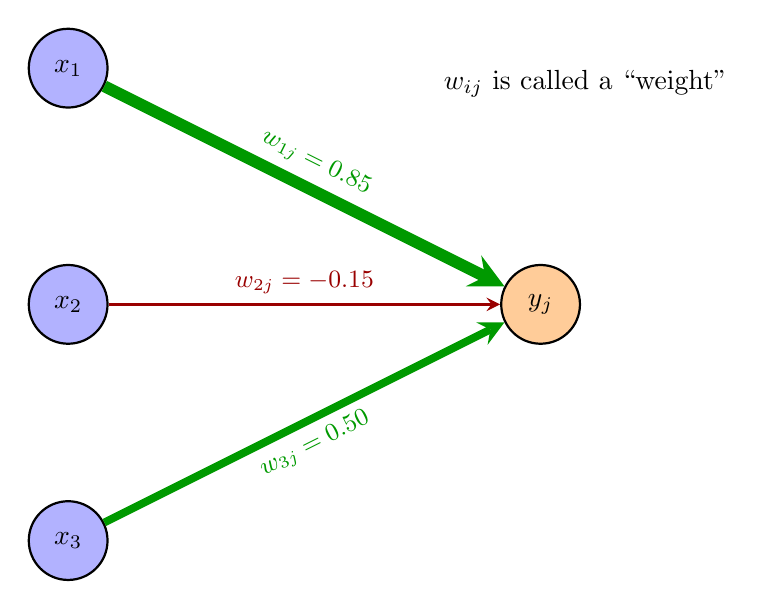
\begin{tikzpicture}[
            neuron/.style={circle, draw=black, fill=white, minimum size=1cm, thick},
            input neuron/.style={neuron, fill=blue!30},
            output neuron/.style={neuron, fill=orange!40},
            strong pos/.style={green!60!black, line width=1.5mm, ->, >=stealth},
            medium pos/.style={green!60!black, line width=1mm, ->, >=stealth},
            weak neg/.style={red!60!black, line width=0.4mm, ->, >=stealth},
            label/.style={font=\small}
        ]

        % Input neurons (left column)
        \node[input neuron] (N1) at (0,3) {$x_1$};
        \node[input neuron] (N2) at (0,0) {$x_2$};
        \node[input neuron] (N3) at (0,-3) {$x_3$};

        % Output neuron (right column)
        \node[output neuron] (N4) at (6,0) {$y_j$};

        
        \node[anchor=south east, font=\normalsize] at (8.5, 2.5) {$w_{ij}$ is called a ``weight''};

        % Connections with weights
        \draw[strong pos] (N1) -- node[label, above, sloped] {$w_{1j} = 0.85$} (N4);
        \draw[weak neg] (N2) -- node[label, above] {$w_{2j} = -0.15$} (N4);
        \draw[medium pos] (N3) -- node[label, below, sloped] {$w_{3j} = 0.50$} (N4);

    \end{tikzpicture}

\end{frame}

\begin{frame}
    
    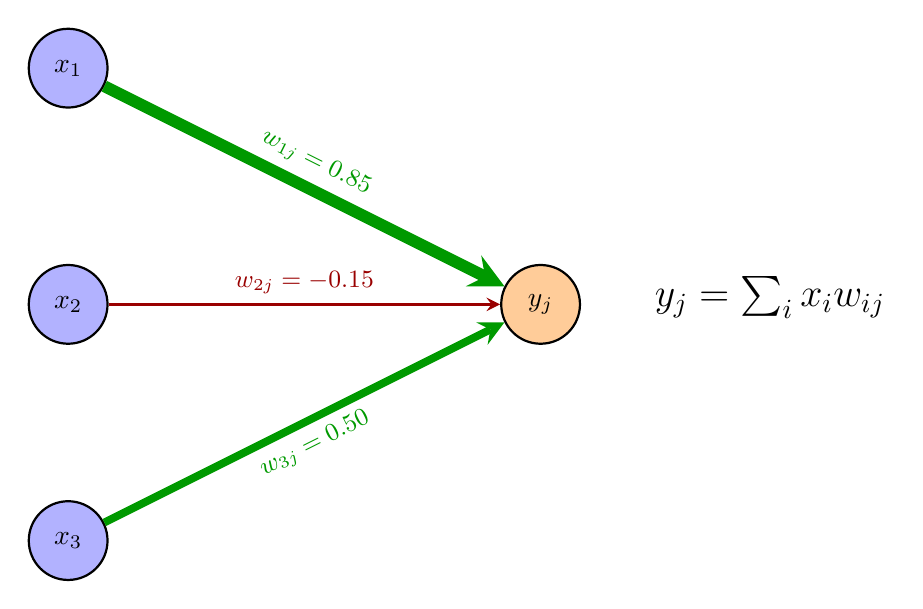
\begin{tikzpicture}[
            neuron/.style={circle, draw=black, fill=white, minimum size=1cm, thick},
            input neuron/.style={neuron, fill=blue!30},
            output neuron/.style={neuron, fill=orange!40},
            strong pos/.style={green!60!black, line width=1.5mm, ->, >=stealth},
            medium pos/.style={green!60!black, line width=1mm, ->, >=stealth},
            weak neg/.style={red!60!black, line width=0.4mm, ->, >=stealth},
            label/.style={font=\small}
        ]

        % Input neurons (left column)
        \node[input neuron] (N1) at (0,3) {$x_1$};
        \node[input neuron] (N2) at (0,0) {$x_2$};
        \node[input neuron] (N3) at (0,-3) {$x_3$};

        % Output neuron (right column)
        \node[output neuron] (N4) at (6,0) {$y_j$};

        
        \node[anchor=south east, font=\Large] at (10.5, -0.3)
            {$y_j = \sum_i  x_i w_{ij}$};

        % Connections with weights
        \draw[strong pos] (N1) -- node[label, above, sloped] {$w_{1j} = 0.85$} (N4);
        \draw[weak neg] (N2) -- node[label, above] {$w_{2j} = -0.15$} (N4);
        \draw[medium pos] (N3) -- node[label, below, sloped] {$w_{3j} = 0.50$} (N4);

    \end{tikzpicture}

\end{frame}

\begin{frame}
    
    % Neural Network with 3 input neurons and 2 output neurons
% To be included in an existing LaTeX document
% Required packages: tikz

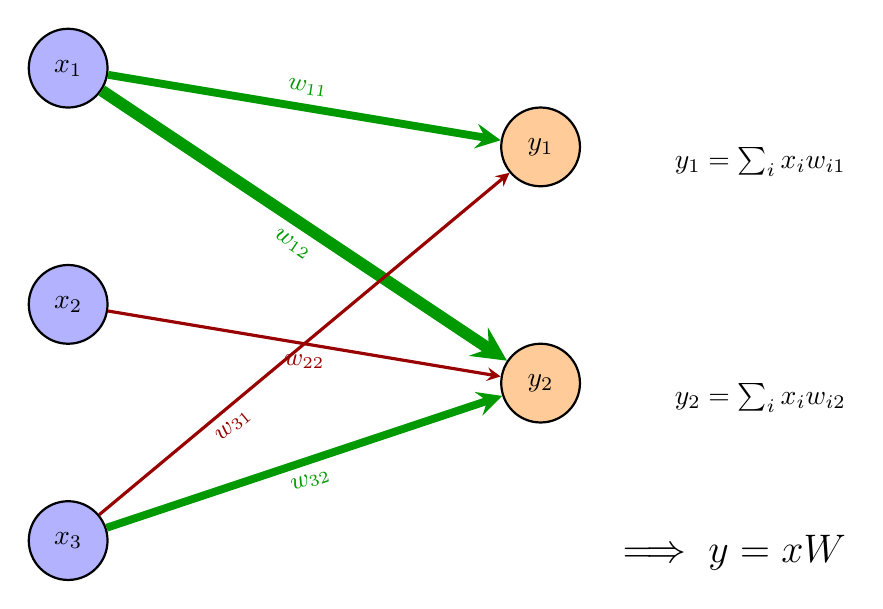
\begin{tikzpicture}[
        neuron/.style={circle, draw=black, fill=white, minimum size=1cm, thick},
        input neuron/.style={neuron, fill=blue!30},
        output neuron/.style={neuron, fill=orange!40},
        strong pos/.style={green!60!black, line width=1.5mm, ->, >=stealth},
        medium pos/.style={green!60!black, line width=1mm, ->, >=stealth},
        weak neg/.style={red!60!black, line width=0.4mm, ->, >=stealth},
        label/.style={font=\small}
    ]

    % Input neurons (left column)
    \node[input neuron] (N1) at (0,3) {$x_1$};
    \node[input neuron] (N2) at (0,0) {$x_2$};
    \node[input neuron] (N3) at (0,-3) {$x_3$};

    % Output neurons (right column)
    \node[output neuron] (N5) at (6,2) {$y_1$};
    \node[output neuron] (N4) at (6,-1) {$y_2$};

    % Connections with weights to N4
    \draw[strong pos] (N1) -- node[label, below, sloped] {$w_{12}$} (N4);
    \draw[weak neg] (N2) -- node[label, below] {$w_{22}$} (N4);
    \draw[medium pos] (N3) -- node[label, below, sloped] {$w_{32}$} (N4);

    % Some connections to the new neuron N5
    \draw[medium pos] (N1) -- node[label, above, sloped] {$w_{11}$} (N5);
    \draw[weak neg] (N3) -- node[label, below, sloped, pos=0.3] {$w_{31}$} (N5);

    % Text in bottom right
    \node[anchor=south east, font=\normalsize] at (10, 1.5) {$y_1 = \sum_i  x_i w_{i1}$};
    \node[anchor=south east, font=\normalsize] at (10,-1.5) {$y_2 = \sum_i  x_i w_{i2}$};
    \node[anchor=south east, font=\Large] at (10,-3.5) {$\implies y = x W$};

\end{tikzpicture}

\end{frame}


\begin{frame}
    
    Note that we are using row vectors:  $y = x W$

        \vspace{0.5em}
        \vspace{0.5em}
    This is natural given our notation 

    \begin{itemize}
        \item $w_{ij}$ points from $i$ to $j$
        \vspace{0.5em}
        \item hence $y_j = \sum_i x_i w_{ij} $  (total flow of activation to node $j$)
        \vspace{0.5em}
        \item hence $y = x W$
    \end{itemize}

        \vspace{0.5em}
        \vspace{0.5em}
        \vspace{0.5em}
    Also fine to use column vectors --- just transpose $W$

\end{frame}

% \begin{frame}
%     
%   \begin{tikzpicture}[scale=0.9, transform shape]
%     \tikzset{
%         cell/.style={
%             rectangle, 
%             minimum size=1cm, 
%             draw=black,
%             thick,
%             anchor=center
%         },
%         memory cell/.style={
%             rectangle,
%             minimum width=1cm,
%             minimum height=1cm,
%             draw=black,
%             thick,
%             anchor=center
%         },
%         arrow style/.style={-{Stealth[scale=1.5]}, thick},
%         label style/.style={font=\small\bfseries}
%     }
%     
%     % Row-major memory layout
%     \begin{scope}[shift={(0,0)}]
%         % 4 CELLS FOR 2x2 MATRIX
%         \node[memory cell] (m0) at (0*1.2,0) {$W_{11}$};
%         \node[memory cell] (m1) at (1*1.2,0) {$W_{12}$};
%         \node[memory cell] (m2) at (2*1.2,0) {$W_{21}$};
%         \node[memory cell] (m3) at (3*1.2,0) {$W_{22}$};
%         
%         % Highlight rows in row-major
%         \begin{scope}[on background layer]
%             \fill[red!10] ($(m0) + (-0.6,-0.6)$) rectangle ($(m1) + (0.6,0.6)$);
%             \fill[blue!10] ($(m2) + (-0.6,-0.6)$) rectangle ($(m3) + (0.6,0.6)$);
%         \end{scope}
%         
%         % Label to the right
%         \node[right=0.8cm of m3, font=\large\bfseries] {row-major storage};
%     \end{scope}
%     
%     % Matrix definition - POSITIONED IN THE MIDDLE and using manual positioning
%     \begin{scope}[shift={(0,-3.5)}]
%         % Create matrix W manually without the matrix library
%         \node[cell] (W11) at (0,0) {$W_{11}$};
%         \node[cell] (W12) at (1,0) {$W_{12}$};
%         \node[cell] (W21) at (0,-1) {$W_{21}$};
%         \node[cell] (W22) at (1,-1) {$W_{22}$};
%     \end{scope}
%     
%     % Column-major memory layout
%     \begin{scope}[shift={(0,-7)}]
%         % 4 CELLS FOR 2x2 MATRIX
%         \node[memory cell] (c0) at (0*1.2,0) {$W_{11}$};
%         \node[memory cell] (c1) at (1*1.2,0) {$W_{21}$};
%         \node[memory cell] (c2) at (2*1.2,0) {$W_{12}$};
%         \node[memory cell] (c3) at (3*1.2,0) {$W_{22}$};
%         
%         % Highlight columns in column-major
%         \begin{scope}[on background layer]
%             \fill[red!10] ($(c0) + (-0.6,-0.6)$) rectangle ($(c1) + (0.6,0.6)$);
%             \fill[blue!10] ($(c2) + (-0.6,-0.6)$) rectangle ($(c3) + (0.6,0.6)$);
%         \end{scope}
%         
%         % Label to the right
%         \node[right=0.8cm of c3, font=\large\bfseries] {column-major storage};
%     \end{scope}
%     
%     % Draw arrows from matrix to row-major memory layout
%     \draw[arrow style, red!60] (W11.north) to[out=90, in=270] (m0.south);
%     \draw[arrow style, red!60] (W12.north) to[out=90, in=270] (m1.south);
%     \draw[arrow style, blue!60] (W21.north) to[out=90, in=270] (m2.south);
%     \draw[arrow style, blue!60] (W22.north) to[out=90, in=270] (m3.south);
%     
%     % Draw arrows from matrix to column-major memory layout
%     % \draw[arrow style, red!60, dashed] (W11.south) to[out=270, in=90] (c0.north);
%     % \draw[arrow style, red!60, dashed] (W21.south) to[out=270, in=90] (c1.north);
%     % \draw[arrow style, blue!60, dashed] (W12.south) to[out=270, in=90] (c2.north);
%     % \draw[arrow style, blue!60, dashed] (W22.south) to[out=270, in=90] (c3.north);
%     
%   \end{tikzpicture}
%
% \end{frame}
%
% \begin{frame}
%     
%   \begin{tikzpicture}[scale=0.9, transform shape]
%     % Define styles
%     \tikzset{
%         cell/.style={
%             rectangle, 
%             minimum size=1cm, 
%             draw=black,
%             thick,
%             anchor=center
%         },
%         memory cell/.style={
%             rectangle,
%             minimum width=1cm,
%             minimum height=1cm,
%             draw=black,
%             thick,
%             anchor=center
%         },
%         arrow style/.style={-{Stealth[scale=1.5]}, thick},
%         label style/.style={font=\small\bfseries}
%     }
%     
%     % Row-major memory layout
%     \begin{scope}[shift={(0,0)}]
%         % 4 CELLS FOR 2x2 MATRIX
%         \node[memory cell] (m0) at (0*1.2,0) {$W_{11}$};
%         \node[memory cell] (m1) at (1*1.2,0) {$W_{12}$};
%         \node[memory cell] (m2) at (2*1.2,0) {$W_{21}$};
%         \node[memory cell] (m3) at (3*1.2,0) {$W_{22}$};
%         
%         % Highlight rows in row-major
%         \begin{scope}[on background layer]
%             \fill[red!10] ($(m0) + (-0.6,-0.6)$) rectangle ($(m1) + (0.6,0.6)$);
%             \fill[blue!10] ($(m2) + (-0.6,-0.6)$) rectangle ($(m3) + (0.6,0.6)$);
%         \end{scope}
%         
%         % Label to the right
%         \node[right=0.8cm of m3, font=\large\bfseries] {row-major storage};
%     \end{scope}
%     
%     % Matrix definition - POSITIONED IN THE MIDDLE and using manual positioning
%     \begin{scope}[shift={(0,-3.5)}]
%         % Create matrix W manually without the matrix library
%         \node[cell] (W11) at (0,0) {$W_{11}$};
%         \node[cell] (W12) at (1,0) {$W_{12}$};
%         \node[cell] (W21) at (0,-1) {$W_{21}$};
%         \node[cell] (W22) at (1,-1) {$W_{22}$};
%     \end{scope}
%     
%     % Column-major memory layout
%     \begin{scope}[shift={(0,-7)}]
%         % 4 CELLS FOR 2x2 MATRIX
%         \node[memory cell] (c0) at (0*1.2,0) {$W_{11}$};
%         \node[memory cell] (c1) at (1*1.2,0) {$W_{21}$};
%         \node[memory cell] (c2) at (2*1.2,0) {$W_{12}$};
%         \node[memory cell] (c3) at (3*1.2,0) {$W_{22}$};
%         
%         % Highlight columns in column-major
%         \begin{scope}[on background layer]
%             \fill[red!10] ($(c0) + (-0.6,-0.6)$) rectangle ($(c1) + (0.6,0.6)$);
%             \fill[blue!10] ($(c2) + (-0.6,-0.6)$) rectangle ($(c3) + (0.6,0.6)$);
%         \end{scope}
%         
%         % Label to the right
%         \node[right=0.8cm of c3, font=\large\bfseries] {column-major storage};
%     \end{scope}
%     
%     % Draw arrows from matrix to row-major memory layout
%     % \draw[arrow style, red!60] (W11.north) to[out=90, in=270] (m0.south);
%     % \draw[arrow style, red!60] (W12.north) to[out=90, in=270] (m1.south);
%     % \draw[arrow style, blue!60] (W21.north) to[out=90, in=270] (m2.south);
%     % \draw[arrow style, blue!60] (W22.north) to[out=90, in=270] (m3.south);
%     
%     % Draw arrows from matrix to column-major memory layout
%     \draw[arrow style, red!60, dashed] (W11.south) to[out=270, in=90] (c0.north);
%     \draw[arrow style, red!60, dashed] (W21.south) to[out=270, in=90] (c1.north);
%     \draw[arrow style, blue!60, dashed] (W12.south) to[out=270, in=90] (c2.north);
%     \draw[arrow style, blue!60, dashed] (W22.south) to[out=270, in=90] (c3.north);
%     
%   \end{tikzpicture}
%
% \end{frame}
%
%
% \begin{frame}[fragile]
%
% Computing $y = xW$ 
%     
%     \begin{minted}{python}
% for i in range(n):     
%     for j in range(m):
%         # Access row elements of W contiguously
%         y[j] += W[i, j] * x[i] 
%     \end{minted}
%
%
%         \vspace{0.5em}
%         \vspace{0.5em}
% Computing $y = Wx$
%
%     \begin{minted}{python}
% for j in range(n):   
%     for i in range(m):
%         # Non-contiguous access of W
%         y[i] += W[i, j] * x[j]        
%     \end{minted}
%
% \end{frame}
%

\begin{frame}{Next steps}

        \vspace{0.5em}
        \vspace{0.5em}
    After computing $y_j = \sum_i x_i w_{ij}$ we 
    \medskip
    %
    \begin{enumerate}
        \item add a bias term $b_j$ and
        \vspace{0.5em}
        \item apply a nonlinear ``activation function'' $\sigma \colon \RR \to \RR$
    \end{enumerate}
    
    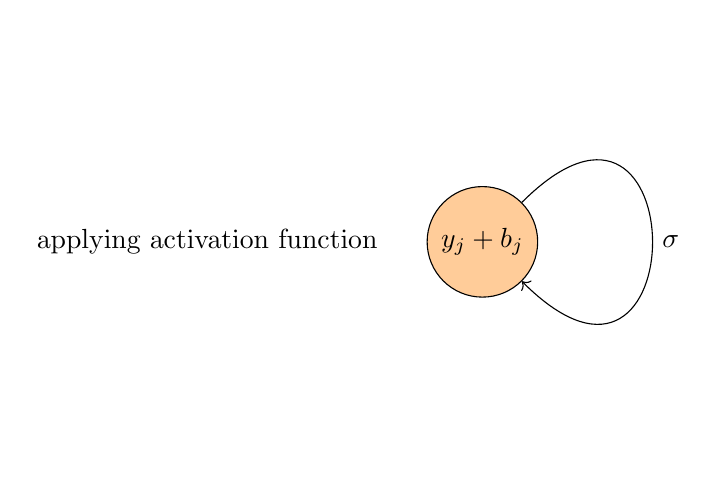
\begin{tikzpicture}
    % Define the node with beige fill
    \node[circle, draw, fill=orange!40, minimum size=0.8cm] (y) {$y_j + b_j$};
    
    % Add text to the left of the node
    \node[left=0.5cm of y] {applying activation function};
    
    % Create the self-loop
    \draw[->] (y) to[out=45, in=-45, looseness=8] node[right] {$\sigma$} (y);
\end{tikzpicture}

\end{frame}

\begin{frame}
    
    First add bias:

    \begin{equation*}
        y_j = \sum_i x_i w_{ij}        
        \qquad \to \qquad
        y_j = \sum_i  x_i w_{ij} + b_j
    \end{equation*}

    Then apply activation:
    %
    \begin{equation*}
        y_j = \sum_i x_i w_{ij} + b_j
        \qquad \to \qquad
        y_j = \sigma \left(\sum_i x_i w_{ij} + b_j \right)
    \end{equation*}

    Applying $\sigma$ pointwise, we can write this in vector form as
    
    \begin{equation*}
        y = \sigma(x W + b)
    \end{equation*}

    
\end{frame}

\begin{frame}{Common activation functions}
    
    \begin{figure}
       \centering
       \scalebox{0.54}{\includegraphics[trim={0cm 0cm 0cm 0cm},clip]{activations.pdf}}
    \end{figure}

\end{frame}

\begin{frame}{Definition of an ANN}

    Let's now put this together
    
    \medskip

    An ANN is a function $f_\theta$ from $\RR^n$ to $\RR^m$ having the form
    %
    \begin{equation*}
        f_\theta
        = G_{m} \circ G_{m-1} \circ \cdots \circ G_{2}  \circ G_{1}
    \end{equation*}
    %
    where
    %
    \begin{itemize}
        \vspace{0.5em}
        \item $\sigma_\ell$ is an activation function
        \vspace{0.5em}
        \item $\theta := \{W_1, b_1, W_2, b_2, \ldots, W_m, b_m\}$
        \vspace{0.5em}
        \item $G_{\ell} (x) = \sigma_\ell(x W_\ell + b_\ell)$ 
    \end{itemize}

\end{frame}


\begin{frame}{Universal function approximation I}

    \textbf{Theorem}. (Cybenko--Hornik 1989, 1991) Let 
    %
    \begin{itemize}
        \item $K \subset \RR^n$ be compact, 
        \item $f$ be a continuous functions from $K$ to $\RR^m$, and
        \item $\sigma$ be a continuous map from $\RR$ to itself
    \end{itemize}

    \medskip
    If $\sigma$ is not polynomial, then, for every $\varepsilon > 0$, 
    there exist an ANN $f_\theta \colon \RR^n \to \RR^m$  such that
    %
    \begin{equation*}
        \sup_{x \in K} \left\| f(x) - f_\theta(x) \right\| 
        < \varepsilon
    \end{equation*}
    %

\end{frame}


\begin{frame}{Universal function approximation II}

    Recall that the ReLU activation has the form $\sigma(x) = \max\{x, 0 \}$

    \medskip
    \medskip

    \textbf{Theorem}. Let 
    %
    \begin{itemize}
        \item $f \colon \RR^n \to \RR^m$ be Borel measurable and
        \item $d = \max\{n+1,m\}$
    \end{itemize}

    \medskip
    If $f$ is Bochner–Lebesgue integrable, then, for any $\varepsilon > 0$,
    there exists a fully connected ReLU network $g$ of width $d$ 
    satisfying 
    %
    \begin{equation*}
        \int \|f(x) - g(x)\| \diff x < \varepsilon
    \end{equation*}
    %

\end{frame}


\begin{frame}
    
    Before we get too excited: many function classes have the universal function
    approximation property

            \vspace{0.4em}
    \begin{itemize}
        \item \brown{polynomials} in $C_0(K) :=$ continuous functions on compacts 
            \vspace{0.4em}
        \item \brown{linear span of an ONS} in a Hilbert space
            \vspace{0.4em}
        \item \brown{SVMs} with RBF kernels in reproducing kernel Hilbert space
            \vspace{0.4em}
        \item \brown{Gaussian processes} with RBF kernels in $C_0(K)$
            \vspace{0.4em}
        \item \brown{random forests}
            \vspace{0.4em}
        \item etc.
    \end{itemize}

\end{frame}


\section{Training ANNs}

\begin{frame}{Training}
    
    \begin{figure}
       \centering
       \scalebox{0.54}{\includegraphics[trim={0cm 0cm 0cm 0cm},clip]{fit_func.pdf}}
    \end{figure}

\end{frame}


\begin{frame}
    

    An ANN is just a particular function $f_\theta$

    \medskip
    We want an ANN that is good at ``prediction''

    \medskip
    Steps
    %
    \begin{enumerate}
        \item Observe data
        \item Adjust the parameter vector $\theta$ to ``fit'' the data
    \end{enumerate}

    \medskip
    \medskip
    Let's clarify these ideas

\end{frame}

\begin{frame}
    
    Suppose we wish to to predict output $y$ from input $x$
    %
    \begin{itemize}
        \item $x \in \RR^k$
        \vspace{0.5em}
        \item $y \in \RR$  (regression problem, scalar output, for simplicity)
    \end{itemize}

    \Egs
    %
    \begin{itemize}
        \item $x = $ cross section of returns, $y = $ return on oil futures tomorrow
        \vspace{0.5em}
        \item $x = $ weather sensor data, $y = $ max temp tomorrow
    \end{itemize}
        \vspace{0.5em}
        \vspace{0.5em}

    Problem:

    \begin{itemize}
        \item observe $(x_i, y_i)_{i=1}^n$ and seek $f$ such that $y_{n+1}
            \approx f(x_{n+1})$
    \end{itemize}


\end{frame}



\begin{frame}

    \boldteal{Nonlinear regression}: Choose parametric class
    $\{f_\theta\}_{\theta \in \Theta}$ and minimize 
    %
    \begin{equation*}
        \ell(\theta) := \frac{1}{n}\sum_{i=1}^n (y_i - f_\theta(x_i))^2
    \end{equation*}


    \pause
    \vspace{0.5em}
    \vspace{0.5em}
    \boldteal{Deep learning}: Nonlinear regression when $\{f_\theta\}$ is a
    class of ANNs:

    %
    \begin{equation*}
        f_\theta
        = G_{m} \circ G_{m-1} \circ \cdots \circ G_{2}  \circ G_{1}
    \end{equation*}
    %
    where
    %
    \begin{itemize}
        \item $G_{\ell} (x) = \sigma_\ell(x W_\ell + b_\ell)$ 
        \vspace{0.5em}
        \item $\theta := \{W_1, b_1, W_2, b_2, \ldots, W_m, b_m\}$
        \vspace{0.5em}
        \item $\sigma_\ell$ is an activation function
    \end{itemize}

\end{frame}

\begin{frame}

    Minimizing the loss functions  
    
    \begin{figure}
       \begin{center}
        \scalebox{0.32}{\includegraphics{gradient_steepest_ascent.png}}
       \end{center}
    \end{figure}

\end{frame}


\begin{frame}{Gradient descent}

    Algorithm: Implement $\nabla \ell$ and then update guess $\theta_k$ via
    
    \begin{equation*}
        \theta_{k+1} = \theta_k - \lambda_k \cdot \nabla \ell(\theta_k)
    \end{equation*}

    \begin{itemize}
        \item take a step in the opposite direction to the grad vector
        \vspace{0.5em}
        \item $\lambda_k$ is the \boldbrown{learning rate} 
        \vspace{0.5em}
        \item iterate until hit a stopping condition
        \vspace{0.5em}
        \item in practice replace $\ell(\theta)$ with batched loss $\to$
            \boldbrown{SGD}
            %
            \begin{equation*}
                \frac{1}{|B|}\sum_{i \in B} (y_i - f_\theta(x_i))^2
            \end{equation*}
    \end{itemize}


\end{frame}



\begin{frame}{Extensions}


    \begin{itemize}
        \item Many variations on SGD
        \vspace{0.5em}
        \item Loss functions with regularization
        \vspace{0.5em}
        \item Cross-entropy loss (classification)
        \vspace{0.5em}
        \item Convolutional neural networks (image processing)
        \vspace{0.5em}
        \item Recurrent neural networks (sequential data)
        \vspace{0.5em}
        \item Transformers (LLMs)
        \vspace{0.5em}
        \item etc.
    \end{itemize}
    
\end{frame}


\section{Why do they work?}

\begin{frame}{Why do they work?}

    Why does DL work so well in so many cases??

    \medskip
    \medskip
    \medskip
    
    Related question: what about overfitting?

\end{frame}


\begin{frame}
    
    \begin{figure}
       \centering
       \scalebox{0.3}{\includegraphics[trim={0cm 0cm 0cm 0cm},clip]{overfit.pdf}}
    \end{figure}

\end{frame}

\begin{frame}
    
    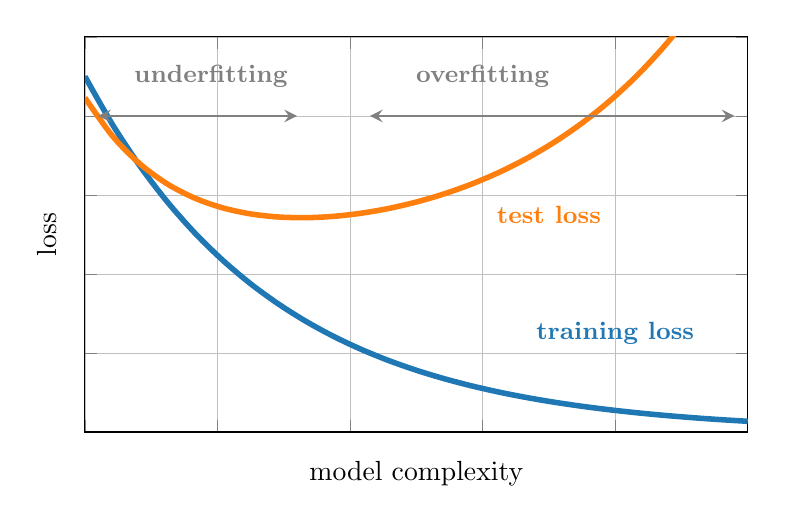
\begin{tikzpicture}
    \begin{axis}[
        width=10cm,
        height=6.6cm,
        xlabel={model complexity},
        ylabel={loss},
        xmin=0, xmax=10,
        ymin=0, ymax=1,
        xticklabels={,,,,,,,,,,},
        yticklabels={,,,,,},
        ylabel near ticks,
        xlabel near ticks,
        legend style={at={(0.97,0.03)}, anchor=south east, draw=none, fill=white, fill opacity=0.7, text opacity=1},
        grid=both,
        grid style={line width=.1pt, draw=gray!10},
        major grid style={line width=.2pt,draw=gray!50},
        every axis plot/.append style={thick},
        title style={font=\large},
        domain=0:10,
        smooth,
    ]

    % Training error curve (monotonically decreasing)
    \addplot[color={rgb,255:red,31; green,119; blue,180}, line width=2pt, name path=training] {0.9*exp(-0.35*x) + 0.0};

    % Test error curve (U-shaped)
    \addplot[color={rgb,255:red,255; green,127; blue,14}, line width=2pt, name path=test] {0.4*exp(-0.7*x) + 0.15*exp(0.35*(x-5)) + 0.42};

    % curve labels
    \node[color={rgb,255:red,31; green,119; blue,180}, font=\small\bfseries] at (axis cs:8,0.25) {training loss};
    \node[color={rgb,255:red,255; green,127; blue,14}, font=\small\bfseries] at (axis cs:7,0.55) {test loss};

    % Underfitting and overfitting regions
    \draw[<->, >=stealth, gray, line width=1pt] (axis cs:3.2,0.8) -- (axis cs:0.2,0.8);
    \node[align=center, gray, font=\small\bfseries] at (axis cs:1.9, 0.9) {underfitting};

    \draw[<->, >=stealth, gray, line width=1pt] (axis cs:4.3,0.8) -- (axis cs:9.8,0.8);
    \node[align=center, gray, font=\small\bfseries] at (axis cs:6, 0.9) {overfitting};

    % Fill regions
    % \path[name path=axis] (axis cs:0,0) -- (axis cs:10,0);
    % \addplot[blue!10, opacity=0.5] fill between[of=axis and training, soft clip={domain=0:3.2}];
    % \addplot[red!10, opacity=0.5] fill between[of=axis and test, soft clip={domain=3.2:10}];
    %
    \end{axis}

    \end{tikzpicture}

\end{frame}


\begin{frame}
    
    If production-level DL models are so large, why don't they overfit?

        \vspace{0.5em}
        \vspace{0.5em}
        \vspace{0.5em}

    \emp{Answer 1} Underlying relationships are complex -- need complex model

        \vspace{0.5em}
        \vspace{0.5em}
    \emp{Answer 2} Engineers avoid using full complexity of the model

    \begin{itemize}
        \item E.g., early stopping halts training when test loss starts to rise
    \end{itemize}


\end{frame}

\begin{frame}
    
    \textbf{Answer 3} Adding randomization prevents overfitting

    \begin{itemize}
        \item E.g., DropConnect and Stochastic Depth
        \vspace{0.5em}
        \item Stochastic gradient descent injects randomness
    \end{itemize}

        \vspace{0.5em}
        \vspace{0.5em}

    Randomness ``adds some smoothing'' to a given data set

        \vspace{0.5em}
    ``The model must learn to be robust to these perturbations, which encourages
    it to find smoother, more generalizable decision boundaries rather than
    fitting to noise in the training data.'' 



\end{frame}


\begin{frame}
    
    \textbf{Answer 4} Modern architectures have inductive biases built in

            \vspace{0.5em}
            \vspace{0.5em}

    \Egs

    \begin{itemize}
        \item Translation invariance in CNNs 
            \vspace{0.5em}
        \item Localization in CNNs -- pixels influenced more by neighbor pixels 
            \vspace{0.5em}
        \item Parameter sharing in RNNs -- similarity of transformations across
            time
    \end{itemize}

            \vspace{0.5em}

    \brown{Injection of good priors guides learning}
    
\end{frame}





\begin{frame}{Summary}
    
    Why can DL successfully generalize?

\end{frame}


\begin{frame}{CS story}

    Because 

    \begin{itemize}
        \item based on a model of the human brain! 
        \vspace{0.5em}
        \item A universal function approximator!
        \vspace{0.5em}
        \item Can break the curse of dimensionality!
    \end{itemize}

    \medskip
    \medskip
    \medskip
    \pause

    \begin{center}
        \brown{Really?}
    \end{center}

\end{frame}


\begin{frame}{Claude AI}
    
    ``Traditional methods typically require you to 
    %
    \begin{itemize}
        \item specify the intrinsic dimension, 
    \medskip
        \item choose kernel parameters, or 
    \medskip
        \item make structural assumptions about the manifold 
    \end{itemize}

    \medskip
    Neural networks automatically adapt to 
    intrinsic structure without requiring this prior knowledge''

    \medskip
    \medskip
    \medskip
    \pause

    \begin{center}
        \brown{Really?}
    \end{center}

\end{frame}

\begin{frame}{Alternative story}


    \begin{itemize}
        \item Can understand without advanced math background
        \vspace{0.5em}
        \item Scales well to high dimensions 
        \vspace{0.5em}
        \item Function evaluations are highly parallelizable
        \vspace{0.5em}
        \item Flexible -- can inject inductive biases
        \vspace{0.5em}
        \item Smooth recursive structure suited to calculating gradients
    \end{itemize}

\end{frame}

\begin{frame}

    On top of --- because of --- this:
    
        \vspace{0.5em}
    \begin{itemize}
        \item Has received massive investment from the CS community
            %
            \begin{itemize}
                \vspace{0.3em}
                \item algos
                \vspace{0.3em}
                \item software
                \vspace{0.3em}
                \item hardware
            \end{itemize}
            %
        \vspace{0.5em}
        \item Many incremental improvements to improve regularization 
        \vspace{0.5em}
        \item Steady increase in injection of domain-specific knowledge
            %
            \begin{itemize}
                \vspace{0.3em}
                \item CNNs
                \vspace{0.3em}
                \item RNNs
                \vspace{0.3em}
                \item transformers, etc.
            \end{itemize}
            %
    \end{itemize}

\end{frame}



\section{DL with JAX}

\begin{frame}{DL with JAX}
    
    \begin{figure}
        \centering
        \scalebox{1}{\includegraphics{jax.png}}
    \end{figure}

    \medskip
    \medskip
    \medskip

    ``JAX is a Python library designed for high-performance numerical computing,
    especially machine learning research.''

    ``Its API for numerical functions is based on NumPy.''

    ``Both Python and NumPy are widely used and familiar, making JAX simple,
    flexible, and easy to adopt.''

\end{frame}


\begin{frame}
    
    JAX is more general-purpose than PyTorch or TensorFlow 

    \begin{itemize}
        \item PT and TF both explicitly designed for deep learning
            \medskip
        \item JAX is a platform for scientific computing designed with machine
            learning / AI applications in mind
    \end{itemize}


    \medskip
    \medskip
    \medskip
    \medskip
    DL in JAX on one slide:

\end{frame}



\begin{frame}[fragile]

    \begin{minted}{python}
def f(θ, x, σ=jnp.tanh):
    for W, b in θ:
        x = σ(x @ W + b)
    return x

def loss(θ, x, y):
  return jnp.sum((y - f(θ, x))**2)

loss_gradient = jit(grad(loss))

def train(θ, x_data, y_data, λ=0.01, m=1_000):
    for i in range(m):
        θ = θ - λ * loss_gradient(θ, x_data, y_data)
    return θ
    \end{minted}

\end{frame}

\begin{frame}
    \frametitle{JAX pytrees}

    The previous code imagined $\theta$ as a list of lists

    In practice, we might want to use more sophisticated data structures

    \begin{itemize}
        \item a list of dictionaries?
        \item a dictionary of dictionaries?
        \item a list of namedtuples?
        \item a list of classes?
        \item a list of a dictionary of classes?
    \end{itemize}

    \medskip
    In that case, how would we implement the gradient descent routine above??

\end{frame}


\begin{frame}

    To handle these kinds of situations we can use pytrees
    
    \begin{itemize}
        \item A tree-like data structure built from Python containers
        \vspace{0.5em}
        \item A concept, not a data type
        \vspace{0.5em}
        \item Used to store parameters
    \end{itemize}

    \vspace{0.5em}
    \vspace{0.5em}
    \Egs

    \begin{itemize}
        \item A list of dictionaries, each dictionary contains parameters
        \item A dictionary of lists 
        \item A dictionary of lists of dictionaries
        \item etc.
    \end{itemize}

\end{frame}




\begin{frame}
    
    
    \resizebox{0.9\textwidth}{!}{
        \input{pytree_fig}
    }

\end{frame}


\begin{frame}
    
    JAX can

    \begin{itemize}
        \item apply functions to all leaves in a pytrees structure
        \vspace{0.5em}
        \item differentiate functions with respect to the leaves of pytrees
        \vspace{0.5em}
        \item etc.
    \end{itemize}


\end{frame}

\begin{frame}
    

\begin{figure}
\centering
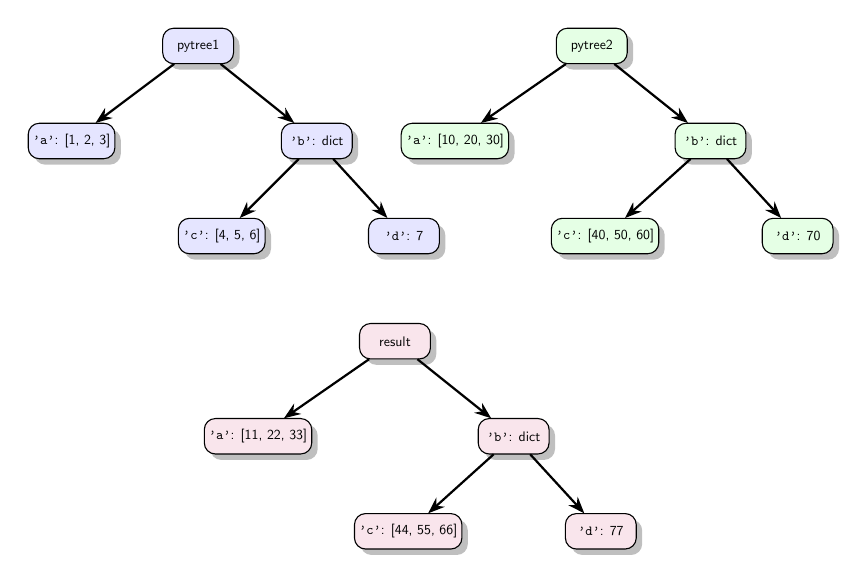
\begin{tikzpicture}[
  scale=0.5, transform shape, % Scale down the entire figure
  level distance=1.5cm,
  level 1/.style={sibling distance=2.5cm},
  level 2/.style={sibling distance=2cm},
  every node/.style={draw, rounded corners, fill=white, drop shadow, align=center, font=\sffamily},
  edge from parent/.style={thick, draw, -{Stealth[length=6pt]}},
  pytree/.style={draw, rounded corners, fill=blue!10, minimum width=1.8cm, minimum height=0.9cm},
  pytree2/.style={draw, rounded corners, fill=green!10, minimum width=1.8cm, minimum height=0.9cm},
  result/.style={draw, rounded corners, fill=purple!10, minimum width=1.8cm, minimum height=0.9cm},
  operation/.style={draw, circle, fill=red!20, inner sep=2pt}
]

% First pytree - unchanged
\node[pytree] (root1) at (-5,0) {pytree1};
\node[pytree, below left=1.5cm and 1.2cm of root1] (a1) {\texttt{'a'}: [1, 2, 3]};
\node[pytree, below right=1.5cm and 1.2cm of root1] (b1) {\texttt{'b'}: dict};
\node[pytree, below left=1.5cm and 0.4cm of b1] (c1) {\texttt{'c'}: [4, 5, 6]};
\node[pytree, below right=1.5cm and 0.4cm of b1] (d1) {\texttt{'d'}: 7};

\draw[edge from parent] (root1) -- (a1);
\draw[edge from parent] (root1) -- (b1);
\draw[edge from parent] (b1) -- (c1);
\draw[edge from parent] (b1) -- (d1);

% Second pytree - unchanged
\node[pytree2] (root2) at (5,0) {pytree2};
\node[pytree2, below left=1.5cm and 1.2cm of root2] (a2) {\texttt{'a'}: [10, 20, 30]};
\node[pytree2, below right=1.5cm and 1.2cm of root2] (b2) {\texttt{'b'}: dict};
\node[pytree2, below left=1.5cm and 0.4cm of b2] (c2) {\texttt{'c'}: [40, 50, 60]};
\node[pytree2, below right=1.5cm and 0.4cm of b2] (d2) {\texttt{'d'}: 70};

\draw[edge from parent] (root2) -- (a2);
\draw[edge from parent] (root2) -- (b2);
\draw[edge from parent] (b2) -- (c2);
\draw[edge from parent] (b2) -- (d2);


% Result pytree - shifted down from -6 to -7.5
\node[result] (rootR) at (0,-7.5) {result};
\node[result, below left=1.5cm and 1.2cm of rootR] (aR) {\texttt{'a'}: [11, 22, 33]};
\node[result, below right=1.5cm and 1.2cm of rootR] (bR) {\texttt{'b'}: dict};
\node[result, below left=1.5cm and 0.4cm of bR] (cR) {\texttt{'c'}: [44, 55, 66]};
\node[result, below right=1.5cm and 0.4cm of bR] (dR) {\texttt{'d'}: 77};

\draw[edge from parent] (rootR) -- (aR);
\draw[edge from parent] (rootR) -- (bR);
\draw[edge from parent] (bR) -- (cR);
\draw[edge from parent] (bR) -- (dR);

% Arrows from input pytrees to result - adjusted for new result position
%\draw[-{Stealth[length=6pt]}, thick, dashed, red] (root1) to[out=-30, in=150] (rootR);
%\draw[-{Stealth[length=6pt]}, thick, dashed, red] (root2) to[out=-150, in=30] (rootR);


\end{tikzpicture}
\caption{\texttt{jax.tree.map(lambda x, y: x + y, pytree1, pytree2)}}
\end{figure}

\end{frame}


\begin{frame}[fragile]
    
    \begin{minted}{python}
def loss_fn(θ, x, y):
    pass  # Details omitted

def sgd_rule(p, g, λ=0.01): 
    return p - λ * g  # Update rule for vectors

# Differentiate the loss function with respect to θ
loss_grad = jit(grad(loss_fn))

# Calculate pytree of gradients at θ
grads = loss_grad(θ, x, y)

# Update all parameters at once
new_θ = jax.tree.map(sgd_rule, θ, grads)
    \end{minted}

\end{frame}




\end{document}


